\documentclass[handout]{beamer}

\usetheme[progressbar=frametitle]{metropolis}
\metroset{block=fill}

\subtitle{NTIN071 Automata and Grammars}
\author{Jakub Bulín (KTIML MFF UK)}

\date{Spring 2025\\ 
    \vspace{1in} 
    \begin{flushleft}
        \it \footnotesize * Adapted from the Czech-lecture slides by Marta Vomlelová with gratitude. The translation, some modifications, and all errors are mine.
    \end{flushleft}
}

%% packages

\usepackage{amsmath}
\usepackage{amssymb}
\usepackage{amsthm}
\usepackage{cancel}
\usepackage{color}
\usepackage{colortbl}
\usepackage{forest}
\usepackage[utf8x]{inputenc}
\usepackage{multicol}
\usepackage{multirow}

%% colors
\definecolor{Gray}{gray}{0.9}

%% TikZ
\usepackage{tikz}
    \usetikzlibrary{
        automata,
        arrows,
        backgrounds,
        decorations.pathmorphing,
        fit,
        positioning,
        shapes,
        shapes.geometric,
        tikzmark
    } 
    \tikzset{>=stealth',shorten >=1pt,auto,node distance=2cm}
    \tikzset{initial text={}}
    \tikzset{elliptic state/.style={draw,ellipse}}

%% amsthm
\theoremstyle{plain}
    \newtheorem*{algorithm}{Algorithm}    
    \newtheorem*{observation}{Observation}
    \newtheorem*{proposition}{Proposition}

\theoremstyle{remark}
    \newtheorem*{exercise}{Exercise}
    \newtheorem*{remark}{Remark}

%% macros
\DeclareMathOperator{\RegE}{RegE}
\DeclareMathOperator{\RL}{RL}

% Just for Lecture 2
\newcommand{\x}{$\times$}
\newcommand{\nx}{\ }



\title{Lecture 6 -- Chomsky Normal Form, Pumping lemma for context-free languages}


\begin{document}


\frame{\titlepage}


\begin{frame}{Recap of Lecture 5}
	
	\begin{itemize}
		\item Grammars: general, context-sensitive, context-free, right-linear (regular) -- Chomsky hierarchy
		\item The language of a grammar, derivation
		\item Right-linear grammars correspond to FA (and so do left/linear)
		\item Linear grammars are stronger
		\item Context-free grammars: parse tree and its yield
		\item (un)ambiguous grammars, inherently ambiguous languages
	\end{itemize}

\end{frame}


\section{2.6 Chomsky Normal Form}


\begin{frame}{Chomsky normal form}
	
	The \alert{Chomsky normal form (ChNF)} of a context-free grammar:
	
	\begin{itemize}
		\item all rules of the form \alert{$A\to BC$} or  \alert{$A\to a$} ($A,B,C\in V$, $a\in T$)
		\item no \alert{useless} symbols
	\end{itemize}

	\begin{theorem}
		For every context-free language $L$ such that $L\setminus \{\epsilon\}\neq \emptyset$ there exists a grammar in ChNF that generates $L\setminus \{\epsilon\}$.
	\end{theorem}
	
	Applications:
	
	\begin{itemize}
		\item Test membership in $L$: the \alert{CYK algorithm} (Sakai 1962) 
		\item Prove the \alert{Pumping lemma for context-free languages}
	\end{itemize}

\end{frame}


\begin{frame}{Converting to ChNF}

	Take any context-free grammar for $L$ and simplify (\alert{in this order!}):
	
	\begin{enumerate}
		\item eliminate \alert{$\epsilon$-productions} $A\to\epsilon$
		\hfill{\small [here we lose $\epsilon\in L$]}
		\item eliminate \alert{unit productions} $A\to B$
		\item eliminate \alert{useless} symbols
		\begin{itemize}
			\item[3a.] \alert{unreachable} \hfill[from the start symbol]
			\item[3b.] \alert{nongenerating} \hfill[a word over terminals]
		\end{itemize} 
	\end{enumerate}

	Now we have a \alert{reduced} grammar. To get to ChNF, we further:
		
	\begin{enumerate}\setcounter{enumi}{3}
		\item \alert{separate} terminals from bodies
		\item \alert{break up} longer bodies
	\end{enumerate}

\end{frame}


\begin{frame}{Step 1: Eliminate $\epsilon$-productions}

	A variable $A\in V$ is \alert{nullable} if $A\Rightarrow^* \epsilon$. An algorithm to find them:
	\begin{itemize}
		\item[\textbf{basis:}] for every $\epsilon$-production $A\to \epsilon$ mark $A$ as nullable
		\item[\textbf{induct:}] if $B\to C_1 \ldots C_k\in\mathcal P$ where all $C_i$ are nullable, $B$ is nullable
	\end{itemize}

	\textbf{To eliminate $\epsilon$-productions:} 1. find nullable variables, 2. remove $\epsilon$-productions, 3. process every production $A\to X_1\ldots X_k \in \mathcal P$:
	\begin{itemize}
		\item let $J\subseteq\{1,\dots,k\}$ be the positions of all nullable variables
		\item for every $J'\subseteq J$ create a copy of the production where $X_j$ for $j\in J'$ are deleted, except if $J=\{1,\dots,k\}$ require $J'\neq\emptyset$
	\end{itemize}

	\textbf{Example:} $\mathcal P=\{S\to AB,A\to aAB\mid\epsilon,B\to ABBA\mid\epsilon\}$

	$S\to AB\mid A\mid B$
	$A\to aAB\mid aA\mid aB\mid a$
	$B\to ABBA\mid ABA\mid ABB\mid BBA\mid AA\mid AB\mid BA\mid BB\mid A\mid B$

\end{frame}


\begin{frame}{Step 2: Eliminate unit productions}

	\textbf{Idea}: for a unit production $A\to B$ copy rules for $B$ with head $A$, but unit productions can be composed, we need transitive closure:

	\alert{Unit pairs} $\mathcal U\subseteq V\times V$ are defined as follows:
	\begin{itemize}
		\item $(A,B)\in\mathcal U$ for every unit production $A\to B\in\mathcal P$
		\item if $(A,B)\in\mathcal U$ and $(B,C)\in\mathcal U$, then $(A,C)\in\mathcal U$
	\end{itemize}

	\textbf{To eliminate unit productions:} 
	\begin{enumerate}
		\item find all unit pairs $\mathcal U$
		\item remove all unit productions
		\item for every unit pair $(A,B)\in\mathcal U$ and production $B\to\mathcal\beta\in\mathcal P$ add the production $A\to\beta$ to $\mathcal P$
	\end{enumerate}

\end{frame}
	

\begin{frame}{Step 2: Eliminate unit productions -- an example}

	$E\to T\mid E+T$\\
	$F\to I\mid (E)$\\
	$I\to a\mid b\mid Ia\mid Ib\mid I0\mid I1$\\
	$T\to F\mid T*F$

	unit pairs:\\		
	$(E,E),(E,F),(E,I),(E,T),$\\
	$(F,F),(F,I),$\\
	$(I,I),$\\
	$(T,F),(T,I),(T,T)$

	the result:\\
	$E\to E+T\mid T*F\mid (E)\mid a\mid b\mid Ia\mid Ib\mid I0\mid I1$
	$I\to a\mid b\mid Ia\mid Ib\mid I0\mid I1$\\
	$F\to (E)\mid a\mid b\mid Ia\mid Ib\mid I0\mid I1$\\
	$T\to T*F\mid (E)\mid a\mid b\mid Ia\mid Ib\mid I0\mid I1$\\
	

\end{frame}


\begin{frame}{Step 3: Eliminate useless symbols}

	\begin{itemize}
		\item $X\in V\cup T$ is a \alert{useful} symbol (in $G$) if there exists a derivation of the form $S\Rightarrow^* \alpha X \beta \Rightarrow^* w$ for some $w \in T^*$
		\item $X$ is \alert{useless} if it is not useful
		\item $X$ is \alert{generating} if $X \Rightarrow^* w$ for some  $w\in T^*$
		\item $X$ is \alert{reachable} if $S\Rightarrow^* \alpha X \beta$ for some $\alpha,\beta\in(V\cup T)^*$
	\end{itemize}

	Observe:
	\begin{itemize}
		\item useful $\Leftrightarrow$ generating and reachable

		\item useless $\Leftrightarrow$ nongenerating or unreachable (we eliminate both)
		\item all terminals are generating
	\end{itemize}

\end{frame}


\begin{frame}{Step 3: Eliminate useless symbols -- the algorithm}

	\begin{enumerate}
		\item Find all generating symbols:
		\begin{itemize}
			\item[\textbf{basis:}] mark all terminals $a\in T$ as generating
			\item[\textbf{induct:}] for every production $A\to\beta$ where every symbol in the body $\beta$ is generating, mark the head $A$ as generating (incl. $A\to \epsilon$)
		\end{itemize}
		\item Remove all \alert{nongenerating} symbols and rules containing them
		\item Find all reachable symbols
		\begin{itemize}
			\item[\textbf{basis:}] mark $S$ as reachable
			\item[\textbf{induct:}] for every production $A\to\beta$ where the head $A$ is reachable mark every symbol in the body $\beta$ as reachable
		\end{itemize}
		\item Remove all \alert{unreachable} symbols and rules containing them		
	\end{enumerate}

	\begin{itemize}
		\item The order is important! Eliminating unreachable symbols can create new nongenerating symbols, but not vice versa.
		\item \textbf{Example:} eliminate nongenerating $B$, then unreachable $A$
		\smallskip
		\begin{center}
			\begin{minipage}{0.25\textwidth}
				$S\to AB\mid a$\\
				$A\to b$
			\end{minipage}
			\begin{minipage}{0.25\textwidth}
				$S\to a$\\
				$A\to b$
			\end{minipage}
			\begin{minipage}{0.25\textwidth}
				$S\to a$
			\end{minipage}
		\end{center}
	\end{itemize}

\end{frame}


\begin{frame}{Steps 4 \& 5: Separate terminals and break up long bodies}

	\textbf{Step 4: Separate terminals from bodies}

	For every terminal $a\in T$, introduce a new variable $V_a$.

	For every rule $A\to\beta$ with $|\beta|\geq 2$, replace every terminal $a$ by $V_a$.
	
	\bigskip

	\textbf{Step 5: Break up longer bodies}

	Replace every rule $A\to B_1\dots B_k$ with $k\geq 3$ with:
	\begin{align*}
		A&\to B_1 C_1\\
		C_1&\to B_2 C_2\\
		&\ \,\vdots\\
		C_{k-2}&\to B_{k-1}B_k
	\end{align*}
	where $C_1,\dots,C_{k-2}$ are new variables (only used for this purpose).
	
\end{frame}


\begin{frame}{Conversion to Chomsky Normal Form}

	ChNF: only useful symbols and rules \alert{$A\to BC$} or \alert{$A\to a$}
	
	\begin{theorem}
		For every context-free language $L$ such that $L\setminus \{\epsilon\}\neq \emptyset$ there exists a grammar in ChNF that generates $L\setminus \{\epsilon\}$.
	\end{theorem}
	\begin{proof}
		Take a context-free grammar $G$ for $L$. Modify it by applying steps 1, 2, 3a, 3b, 4, and 5, in order. Clearly, the result is in ChNF. After step 1 we get $G'$ such that $L(G')=L(G)\setminus \{\epsilon\}$; the remaining steps produce equivalent grammars. Steps 2-5 don't add any $\epsilon$-productions, 3-5 don't add unit productions, 3b-5 don't add nongenerating symbols, 4-5 don't add useless, etc.
	\end{proof}

	Note: If we only apply 1, 2, 3a, and 3b, we get a \alert{reduced} grammar: only useful symbols, no $\epsilon$-productions, no unit productions.

\end{frame}


\begin{frame}{Example}

	\begin{multicols}{2}
		
		$I\to a\mid b\mid Ia\mid Ib\mid I0\mid I1$\\
		$F\to I\mid (E)$
		
		$T\to F\mid T*F$\\
		$E\to T\mid E+T$
	\end{multicols}

	\bigskip
	\hrule

	\begin{multicols}{2}
		\small

		\textbf{reduce + separate}

		$I\to a\mid b\mid IA\mid IB\mid IZ\mid IU$\\
		$F\to LER\mid a\mid b\mid IA\mid IB\mid IZ\mid IU$\\
		$T\to TMF\mid LER\mid a\mid b\mid IA\mid IB\mid IZ\mid IU$\\
		$E\to EPT\mid TMF\mid LER\mid a\mid b\mid IA\mid IB\mid IZ\mid IU$\\

		\bigskip
		
		$A\to a$, $B\to b$, $Z\to 0$, $U\to 1$,\\
		$P\to +$, $M\to *$, $L\to ($, $R\to )$
		
		\bigskip\bigskip

		\textbf{break up longer bodies}

		$F\to LC_3\mid a\mid b\mid IA\mid IB\mid IZ\mid IU$\\
		$T\to TC_2\mid LC_3\mid a\mid b\mid IA\mid IB\mid IZ\mid IU$\\
		$E\to EC_1\mid TC_2\mid LC_3\mid a\mid b\mid IA\mid IB\mid IZ\mid IU$\\
		$C_1\to PT$\\
		$C_2\to MF$\\
		$C_3\to ER$\\
		$I,A,B,Z,U,P,M,L,R$ same as on the left side
	\end{multicols}

\end{frame}


\section{2.7 Pumping lemma for context-free languages}


\begin{frame}{Pumping lemma for context-free languages}

	\begin{theorem}[Pumping Lemma for Context Free Languages]
		Let $L\subseteq\Sigma^*$ be context-free. Then there exists $n\in\mathbb N$ s.t. for any $z\in L, |z|\geq n$ there are $u,v,w,x,y\in\Sigma^*$ s.t. $z=uvwxy$ and:
		
		(i) $|vwx|\leq n $ \hfill (ii) $|vx|>0$ \hfill (iii) $uv^iwx^iy\in L$ for all $i\geq 0$
	\end{theorem}

	\textbf{Proof idea:} Take a ChNF grammar for $L$. If $z\in L$ is long enough, a parse tree for $z$ must contain a path from $S$ to a leaf (terminal) of length $|V|+1$. Some nonterminal $N\in V$ repeats on this path giving two subtrees with root $N$: a larger one containing a smaller one. Replace the larger with a copy of the smaller ($i=0$) or the smaller with a copy of the larger ($i=2$).

	\textbf{What is long enough?} If $|z|>2^{k-1}$, then the depth of the tree is $k+1$. (All inner nodes not immediately above a leaf are binary!) 

\end{frame}


\begin{frame}{The proof in a picture}

	\vspace{-6pt}
	\begin{center}
		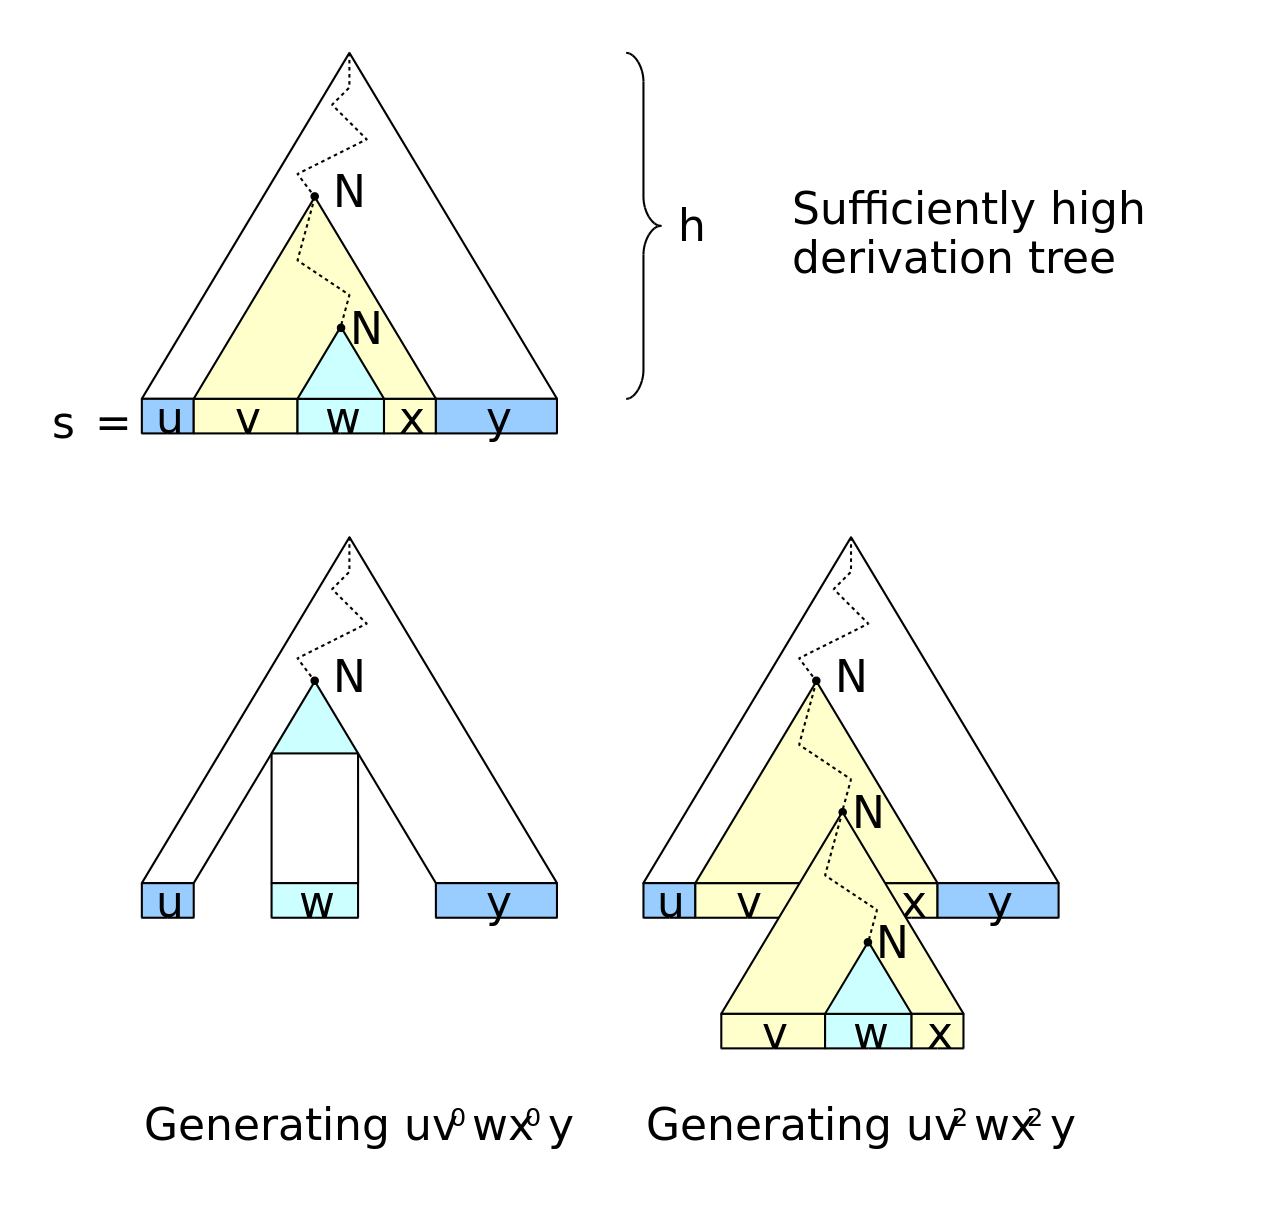
\includegraphics[height=0.92\textheight]{files/pumping-lemma-for-context-free-languages.png}
	\end{center}
	\vspace{-12pt}
	{\footnotesize Image by Jochen Burghardt, CC BY-SA 3.0, from \href{https://en.wikipedia.org/wiki/Pumping_lemma_for_context-free_languages}{Wikipedia}}
		
	
\end{frame}


\begin{frame}{The proof}

	If $L=\emptyset$ and $L=\{\epsilon\}$ trivial, take $n=1$. Otherwise take a ChNF grammar for $L$. Set $n=2^{|V|-1}+1$ . Let $z\in L$ with $|z|\geq n$.
	
	A parse tree for $z$ contains a path from $S$ to a terminal $t$ of length at least $|V|+1$. At least two of the last $|V|+1$ nonterminals on this path must be the same. Let $A^1, A^2$ be such a pair that is closest to $t$. Let $T^1,T^2$ be the subtrees rooted at $A^1, A^2$.
		
	The path from $A^1$ to $t$ is the longest one in $T^1$ and has length at most $(k+1)$. Thus $|vwx|\leq n $.

	There are two paths from $A^1$ (ChNF!): one leads to $T^2$, the other to the rest, it must generate at least one letter (no $\epsilon$-productions). Thus $|vx|>0$.

\end{frame}


\begin{frame}{The proof cont'd}

	The word $z=uvwxy$ is derived as follows:
	\begin{itemize}
		\item $A^2\Rightarrow^* w$
		\item $A^1\Rightarrow^*vA^2x\Rightarrow^* vwx$
		\item $S\Rightarrow^*uA^1y\Rightarrow^*uvA^2xy\Rightarrow^*uvwxy$
	\end{itemize}

	For $i=0$: replace $T^1$ by $T^2$
	$$
	S\Rightarrow^*uA^2y\Rightarrow^*uwy
	$$

	For $i=2$: replace $T^2$ by a copy of $T^1$
	$$
	S\Rightarrow^*uA^1y\Rightarrow^*uvA^1xy\Rightarrow^*uvvA^2xxy\Rightarrow^*uvvwxxy
	$$

	For $i\geq 3$ repeat the above.\hfill\qedsymbol
	
\end{frame}


\begin{frame}{Application: proving a laguage is not context-free}

	\begin{example}
		The language $L=\{0^n1^n2^n\mid n\geq 0\}$ is not context-free.
	\end{example}
	Suppose for contradiction that it is. Let $n$ be constant from the Pumping lemma. Choose $z=0^n1^n2^n\in L$. Clearly $|z|\geq n$.

	The Pumping lemma gives us a split $z=uvwxy$ satisfying (i)--(iii). Since $|vwx|\leq n $, the pumped part $vx$ contains at most two of the symbols $0,1,2$. Pumping will violate equal number of symbols.\hfill\qedsymbol

	\medskip

	\begin{example}
		The language $L=\{0^i1^j2^k\mid 0\leq i\leq j\leq k\}$ is not context-free.
	\end{example}
	Similar as above, also $z=0^n1^n2^n$, at most two symbols pumped:
	\begin{itemize}
		\item if 0 or 1 are pumped, but 2 is not: pump up ($i=2$)
		\item if 1 or 2 are pumped, but 0 is not: pump down ($i=0$)\hfill\qedsymbol

	\end{itemize}
\end{frame}


\begin{frame}{More examples}

	\begin{example}
		$L=\{0^j1^k2^j3^k\mid j,k\geq 0\}$ is not context-free.
	\end{example}		
	Similar as before, choose $z=0^n1^n2^n3^n$, $vx$ must contain some symbol. But from $|vwx|\leq n$ we know that it can contain neither both 0 and 2, nor both 1 and 3. In any case, the equal number of symbols 0 and 2 or 1 and 3 is violated.\hfill\qedsymbol

	\bigskip

	\begin{example}
		$L=\{ww\mid w\in\{0,1\}^*\}$ is not context-free.
	\end{example}	
	Choose $z=0^n1^n0^n1^n$, then $|z|\geq n$. The pumped part can cover neither both blocks of 0s nor both blocks of 1s. Four cases to consider: $vx$ contains a symbol from the 1st block of 0s, 1st block of 1s, 2nd 0s, 2nd 1s. In all cases we get a violation.\hfill\qedsymbol

\end{frame}


\begin{frame}{It is not a characterization}

	The Pumping lemma is again only an implication, not equivalence:

	\begin{example}
		$L=\{a^ib^jc^kd^\ell| i=0 \text{ or } j=k=\ell\}$ can be pumped. But it is not context-free.
	\end{example}
		
	\begin{tabular}{l l}
		$i=0: b^jc^kd^l$ & can be pumped in any letter\\
		$i>0:a^ib^nc^nd^n$ & can be pumped in $a^*$
	\end{tabular}

	\medskip
	
	What to do in such cases?
	\begin{itemize}
		\item \href{https://is.cuni.cz/studium/predmety/index.php?do=predmet&kod=NTIN071}{\alert{Ogden's lemma}}: generalize Pumping lemma, mark some of the letters, some marked symbol is pumped
		\item use closure properties of context-free languages
	\end{itemize}

\end{frame}


\section{2.8 The CYK algorithm}


\begin{frame}{Testing membership in a context-free language}

	Given a context-free grammar $G$ \alert{in Chomsky Normal Form} and a word $w=a_1\dots a_n\in T^*$, determine if $w\in L(G)$.

	\bigskip

	\textbf{Naive, inefficient algorithm:}
	
	Construct all parse trees from $G$ of appropriate depth ($\lceil log_2|w|\rceil$), check if the yield is $w$.

	\bigskip


	\textbf{The Cocke-Younger-Kasami algorithm:} 
	
	Use \alert{dynamic programming} to compute, for every $1\leq i\leq j\leq n$, the set $X_{ij}$ of all variables of $G$ that generate the subword $a_i\dots a_j$.

	Then check if $S\in X_{1n}$.

	(Very efficient, worst-case time complexity $\mathcal O(n^3|G|)$.)

\end{frame}


\begin{frame}{The CYK algorithm}

	\begin{itemize}
		\item \textbf{input:} $G=(V,T,\mathcal P,S)$ in ChNF, $w=a_1\dots a_n\in T^*$
		\item \textbf{decide:} $w\in L(G)$?
	\end{itemize}	
	
	\begin{multicols}{2}
		Compute for $1\leq i\leq j\leq n$:
		
		\vspace{-24pt}
		$$
		X_{ij}=\{A\in V\mid A\Rightarrow^* a_ia_{i+1}\ldots a_j\}
		$$
		\vspace{-24pt}

		using dynamic programming (storing results in a table)
		
		\begin{center}
			\scalebox{0.85}{
				\begin{tabular}{|c c c c c c c c}
					$X_{15}$ \\ 		
					$X_{14}$ &  $X_{25}$  \\ 
					$X_{13}$ &  $X_{24}$ &  $X_{35}$ \\
					$X_{12}$ &  $X_{23}$ & $X_{34}$ &  $X_{45}$ \\ 
					$X_{11}$ & $X_{22}$ &  $X_{33}$ &$X_{44}$ &$X_{55}$ \\ \hline
					\rowcolor{Gray}$a_1$&$a_2$&$a_3$&$a_4$&$a_5$
				\end{tabular}
			}		
		\end{center}		
	\end{multicols}

	\begin{enumerate}
		\item \textbf{Initialize:} $X_{ii}=\{A\in V\mid A\to a_i \in \mathcal P\}$
		\item \textbf{Fill upwards:} $$X_{ij}=\{A\in V\mid A\to BC\in \mathcal P,B\in X_{ik}, C\in X_{k+1,j}\}$$
		\item \textbf{Check:} Is $S\in X_{1n}$?
	\end{enumerate}	

\end{frame}


\begin{frame}{The CYK algorithm: an example}

	\begin{example}
	$G=(\{S,A,B,C\},\{a,b\},\mathcal P,S)$ with $\mathcal P=\{S\to AB\mid BC, A\to BA\mid a, B\to CC\mid b, C\to AB\mid a\}$
	\end{example}
	\vspace{-6pt}
	Rules reversed:\vspace{-6pt}
	\begin{quote}
		\begin{multicols}{4}\small
			$AB  \leftarrow  \{S,C\}$\\
			$BA  \leftarrow  \{A\}$\\
			$BC  \leftarrow  \{S\}$\\
			$CC  \leftarrow  \{B\}$\\
			$b   \leftarrow  \{B\}$\\
			$a   \leftarrow  \{A,C\}$
		\end{multicols}	
	\end{quote}

	\vspace{-12pt}
	Fill upwards:
	\vspace{3pt}

	\begin{center}
		\begin{tabular}{|c c c c c c c c}
			$\{\alert{S},A,C\}$ \\ 
			- &  $\{S,A,C\}$  \\ 
			- &  $\{B\}$ &  $\{B\}$ \\ 
			$\{S,A\}$ &  $\{B\}$ & $\{S,C\}$ &  $\{S,A\}$ \\ 
			$\{B\}$ & $\{A,C\}$ &  $\{A,C\}$ &$\{B\}$ &$\{A,C\}$ \\ %\cline{1-7}
			\rowcolor{Gray}$b$&$a$&$a$&$b$&$a$
		\end{tabular}
	\end{center}
\end{frame}


\end{document}

\begin{frame}{Testing membership in a context-free language}
	
	\begin{example}
		
	\end{example}
	$G=(V,T,P,S)$, $P=\{S \to AB\mid BC, A \to BA\mid a, B\to CC\mid b, C\to AB\mid a\}$
	
	\bigskip
	
	Start filling from the bottom:
	
	\bigskip
	
	\begin{tabular}{|c c c c c c c c}
	 $\{S,A,C\}$ \\ 
	- &  $\{S,A,C\}$  \\ 
	- &  $\{B\}$ &  $\{B\}$ \\ 
	 $\{S,A\}$ &  $\{B\}$ & $\{S,C\}$ &  $\{S,A\}$ \\ 
	 $\{B\}$ & $\{A,C\}$ &  $\{A,C\}$ &$\{B\}$ &$\{A,C\}$ \\ \hline 
	 \rowcolor{Gray}$b$&$a$&$a$&$b$&$a$
	\end{tabular}
	\end{example}


	

\end{frame}


\end{document}
